\documentclass{ctexart}
\usepackage{amsmath}
\usepackage{amssymb}
\usepackage{graphicx}
\usepackage{float}
\usepackage{listings}
\usepackage{booktabs}
\usepackage{pythonhighlight}
\usepackage{enumerate}
\usepackage{subfigure}
\usepackage[a4paper,top=4cm,bottom=4cm,left=4cm,right=4cm,marginparwidth=1.75cm]{geometry}

\title{无线可充电传感器的充电方案}
\date{}

\begin{document}
    \maketitle

    \section*{摘要}
    随着物联网的快速发展,无线传感器网络WSN(Wireless Sensor Network)在生活中的
    应用也越来越广泛。无线传感器网络中包括若干传感器(Sensors)以及一个数据中心(
    Data Center)。传感器从环境中收集信息后每隔一段时间将收集到的信息发送到数据中心
    。数据中心对数据进行分析并回传控制信息。

    为了保证WSN的持续稳定运行,需要用移动充电器对数据中心和传感器充电。由于在路上移
    动充电器会消耗大量的能源,所以如何选择合适的移动路径便成为了一个至关重要的问题。
    
    在第一问中,题目中规定有一台移动充电器,我们考虑到参数较多(有30个地点需要全部经
    过),为了避免指数爆炸,使用了遗传算法。经过不断的选择、交叉和变异,最终得到了最
    后的路线规划,最短路径总长为11601.1m。

    在第二问中,为了简化题目的求解,我们首先合理假设移动充电器每次都将传感器的电池充
    满。如果不充满,那么多余出来的电池容量相当于浪费,所以可认为我们的假设合理。在问
    题求解阶段,我们根据第一问所得的最短路径对29个传感器分别列出约束不等式,进行求解,
    最终得到最后的总约束条件,也就是最小的电池容量。

    在第三问中,此时我们有四台移动充电器可供使用,为了使其发挥应有的效果,我们对第一
    问中的遗传算法作了适当的改进。在基因初始化和选择、交叉、变异等方面均考虑到了充电
    器数量的不同,最终分别得到了四台移动充电器不同的移动路径,进一步减少了移动充电器
    在路程中浪费的资源。在电池最小容量的求解中,我们参照问题二的思路,将四台移动充电
    器先分开求解,最后整合得到结果。
    
    \paragraph{关键词}遗传算法选择;交叉;变异;最短路径;不等式约束
    \newpage

    \section{问题重述}
    为了保证WSN的持续稳定运行,需要用移动充电器对数据中心和传感器充电。这里移动充电
    器的能量消耗包含两部分:传输给传感器的能量以及在充电的路上消耗的能量。显然,传输
    给传感器的能量必需的,而在路上消耗的能量是可以尽量减少的。

    由题可知,在路上消耗的能量与路程总长度成正比:路程越长浪费的能量也就越多。因此,
    为了尽可能节约能量,我们需要尽可能的减少所需的总路程。

    这是第一问和第三问第一部分的主要内容。不同点在于第一问中只有一台移动充电器,第三
    问中有四台移动充电器。如何合理规划移动充电器的路径,以达到最小化总路径是解决问题
    的关键。

    在确定了最短的路径后,电池的容量也是一个十分重要的问题。如何在保证系统稳定运行的
    情况下最大限度地减少电池的容量以减少成本,是第二问和第三问第二部分的主要工作。需
    要结合传感器的能量消耗速率、移动充电器的移动速度等多方面因素进行考虑。


    \section{问题一的建模与求解}
    由题目描述可知,WSN中有1个数据中心和29个传感器,为了保证系统的稳定以运行,现在
    考虑派出一个移动充电器为数据中心和传感器充电。

    移动充电器从数据中心出发,以固定的速度依次经过每个传感器,在每个传感器处停留一段
    时间并以固定的充电速率为传感器充电,直到为所有传感器充电完成之后返回数据中心。每
    个传感器都有特定的能量消耗速率,以及固定的电池容量。移动充电器的能量消耗主要有两
    个方面:一是为传感器节点充电所导致的正常的能量消耗;另外一方面则是移动充电器在去
    为传感器充电的路上的能量消耗。为了减小移动充电器在路上的能量消耗,需要合理地规划
    移动充电器的充电路线。

    这个问题是一个典型的旅行商问题:给定一系列城市和每对城市之间的距离,求解访问每一
    座城市一次并回到起始城市的最短回路。考虑到旅行商问题是一个NP-hard问题,很难用常
    规的算法去求解,或者说,用常规的算法很难计算出结果。为此,我们决定采用启发式算法
    ——遗传算法来解决这一问题。

    \subsection{遗传算法}
    遗传算法是通过模拟生物进化的过程来完成优化搜索的。遗传算法起源于达尔文的进化论,
    是一类借鉴生物界自然选择和自然遗传机制的随机化搜索算法。“优胜劣汰”这一自然规律的
    生物进化过程本身是一个自然的、并行发生的、鲁棒的优化过程,生物种群通过生物体的遗
    传、变异来提高对环境的适应性,从而达到优化的目的。在我们的算法中,主要包含以下几
    个步骤:
    \begin{enumerate}[a]
        \item 参数的设置:确定个体编码方式,这里即为使用节点编号组成路径
        \item 初始随机解的生成:随机生成可行路径,路径中不能有重复节点
        \item 选择算子:选择父代的策略
        \item 交叉算子:交叉父代并产生新个体,同时需要考虑解决节点冲突
        \item 变异算子:对新个体进行变异操作
        \item 保留策略:精英保留或者父代完全不参与子代
    \end{enumerate}

    \subsection{算法细节}
    \subsubsection{基因编码}
    为了给每一个基因编码,我们用0表示数据中心,用$i$表示第$i$个传感器。用包含30个序号
    的数组序列表示一种路线(个体),数组元素的序号表示路径的顺序。数组序列中值不重复,
    即不重复到达某一个传感器。
    \subsubsection{初始化种群}
    随机生成$m$个基因编码序列作为初始种群。
    \subsubsection{评估适应度}
    在该问题中,为了尽可能减少充电器在路上的能量消耗,也就是要尽可能减少路径的总长度(
    这里我们假设移动充电器在路上的平均能量消耗相同)。因此,适应度取值为路径总长度的倒
    数,即$\frac{1}{\mbox{distance}}$。
    \subsubsection{产生新种群}
    产生新种群分为选择、交叉和变异。个体被选中的概率取决于该个体的适应度值,若该个体的
    适应度越高,则其被选中的概率也就越大。

    随机选择两个个体后,以一定的概率交叉,子代分别继承父母的部分基因,且保持顺序与父代
    一致。

    交叉发生之后,变异也以一定的概率发生。在该问题中因为每一个传感器只会经过一次,所以
    在变异的时候不能只是改变基因序列中的某一位的值(这会导致一个传感器经过两次),应该
    随机交换两个位置的值。

    \subsection{最终结果}
    我们将各传感器以及数据中心的经纬度作为参数输入程序,计算出其距离矩阵,再进行遗传算
    法求解,结果如下图所示:
    \begin{figure}[H]
        \centering
        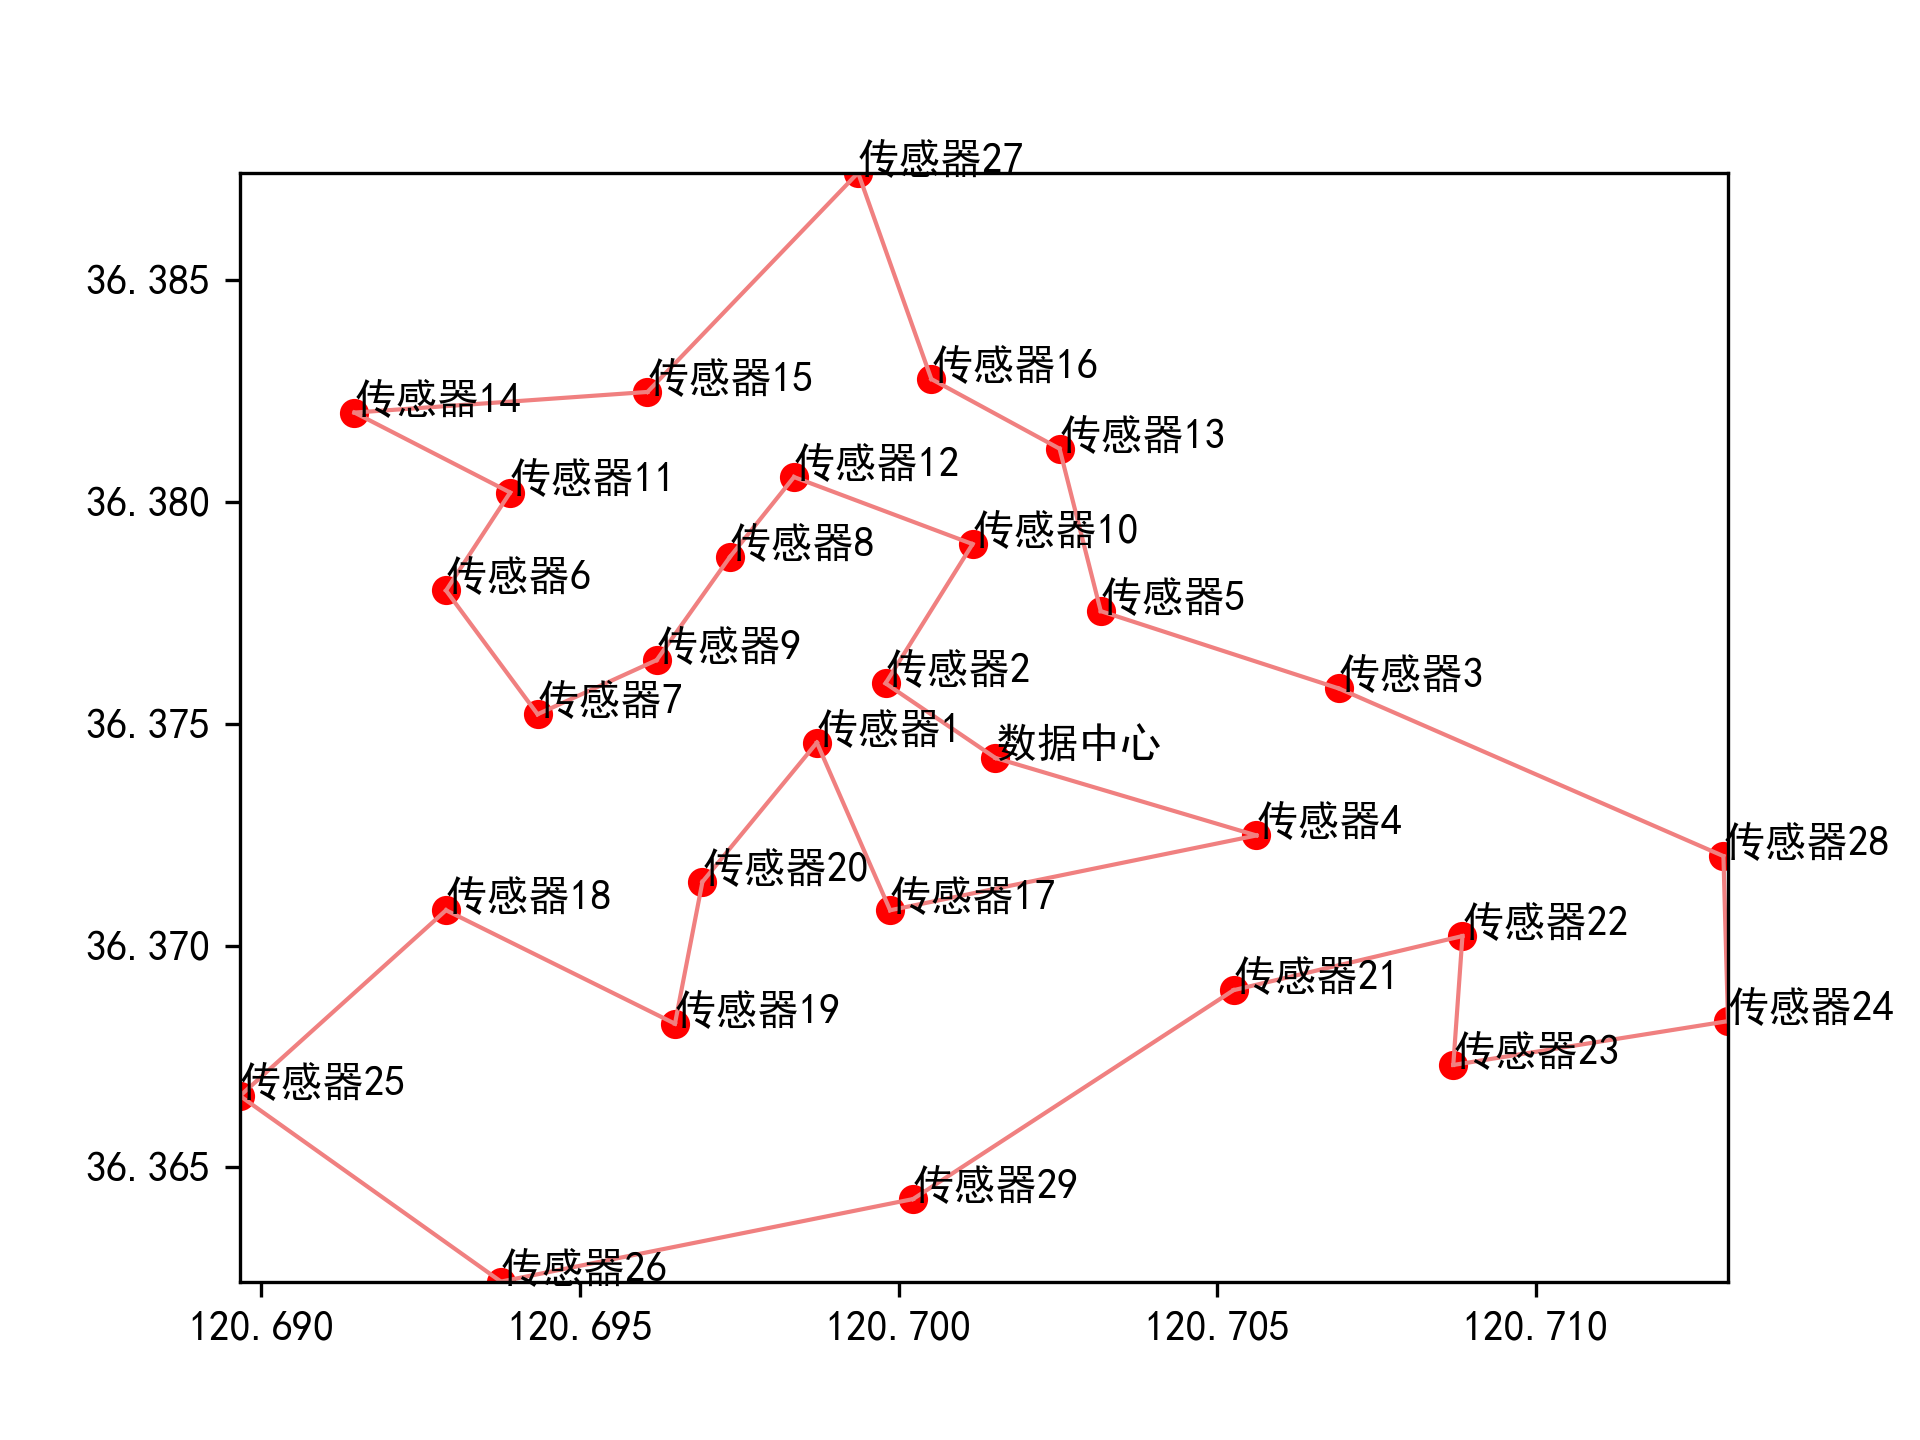
\includegraphics[width=1\textwidth]{figure/path.png}
        \caption {路线安排结果图示}
    \end{figure}

    \subsection{算法的局限性分析}
    遗传算法是一种群体性算法,具有并行性,全局搜索能力极强,局部搜索能力差。参数的选择
    对算法性能影响很大,并且需要对问题进行编码。算法前期收敛较快,但随着迭代次数的增加,
    种群陷入局部较优解,需要长时间的迭代才能继续下降,且越接近最优解越难下降。

    由于遗传算法是一种启发式算法,所以不能保证其达到全局最优解,而是只能达到局部最优解。
    根据多次实验可得,每次的最终结果都有或多或少的差别,收敛性较差,需要后续进行持续改
    进。

    \section{问题二的建模与求解}
    问题二需要在问题一的基础上,进一步对电池容量进行分析。由题目可得,每个传感器的能量
    消耗速率各不相同,但其都需要在剩余电量高于$f(mA)$才能正常工作。为此,我们需要解出
    电池的最小容量,以保证在移动充电器循环对这29个传感器进行充电时,其始终能保持持续稳
    定工作。
    \subsection{约束条件的建立}
    此处的约束条件为,在移动充电器循环为传感器充电时,传感器的剩余电量要始终高于最低工
    作电量。将其转换为数学语言,即对于每一个传感器$x_i$,移动充电器将其充满电后,将去
    给剩余的28个充电器充电以及再次回到$x_i$处,在这段时间内,$x_i$的电量需要保持在最
    低工作电量之上。以此为约束条件对29个传感器分别列出不等式。
    \subsection{求解结果}
    根据问题一中计算得出的路线,最短路径总长为$S=11601.1m$,并代入最大消耗功率速度
    $c_{max}=7.8mA/h$,可得
    \begin{equation}
        C\geq f+\frac{11601.1}{v(\frac{1}{7.8}-\frac{28}{r})}
    \end{equation}
    其中,$C$为每一个传感器的电池容量,$f$为传感器的最低工作电量,$v$为移动充电器的充
    电速度,$r$为移动充电器的充电速率。

    \section{问题三的建模与求解}
    \subsection{问题分析}
    在问题三中,题目引入了一个新的条件:同时派出四台移动充电器来为传感器充电。此时因为
    移动充电器数量的增多,相应的,总路程也会减少。为了得到此时的最有安排,我们依然决定
    采用遗传算法,并对第一问的算法进行适当的修改,使其满足四台移动充电器的需求。
    \subsection{算法修改}
    \subsubsection{基因编码}
    基因编码的方式依然与第一问相同,用数字0~30对数据中心和传感器顺序编码。
    \subsubsection{初始化种群}
    由于此时有四台移动充电器,所以我们需要初始化$m$组基因编码。在每一组基因编码中,分别
    包含四个基因编码,用以代替四台移动充电器的行动路径,且这几条编码均从0开始,也就是从
    数据中心出发。注意,除0之外的其余编码在四条基因中的出现次数有且仅有一次,因为考虑到
    四台移动充电器不可能为同一个传感器充电多余一次(在一次循环中)。

    为了使算法更快地收敛,结合尝试,我们将29个传感器近似四等分,使每一台移动充电器分别负
    责7~8个传感器,也就是使初始化的每条分基因的长度为7或8。
    \subsubsection{评估适应度}
    适应度依然为总距离的倒数,即$\frac{1}{\mbox{distance}}$。
    \subsubsection{产生新种群}
    在产生新种群时,因为每个分基因的长度不定,所以在交叉和变异时需要考虑到它们长度的变化。
    而选择这一步依然与问题一相同。

    在变异时,除去随机交换基因中两个位置的值,还应该按一定的概率增加或减少以为分基因的长
    度,以达到改变基因长度的目的。

    \subsection{最短路径结果}

    \begin{figure}[H]
        \centering
        
        \subfigure[移动充电器1]{
        \begin{minipage}[t]{0.5\linewidth}
        \centering
        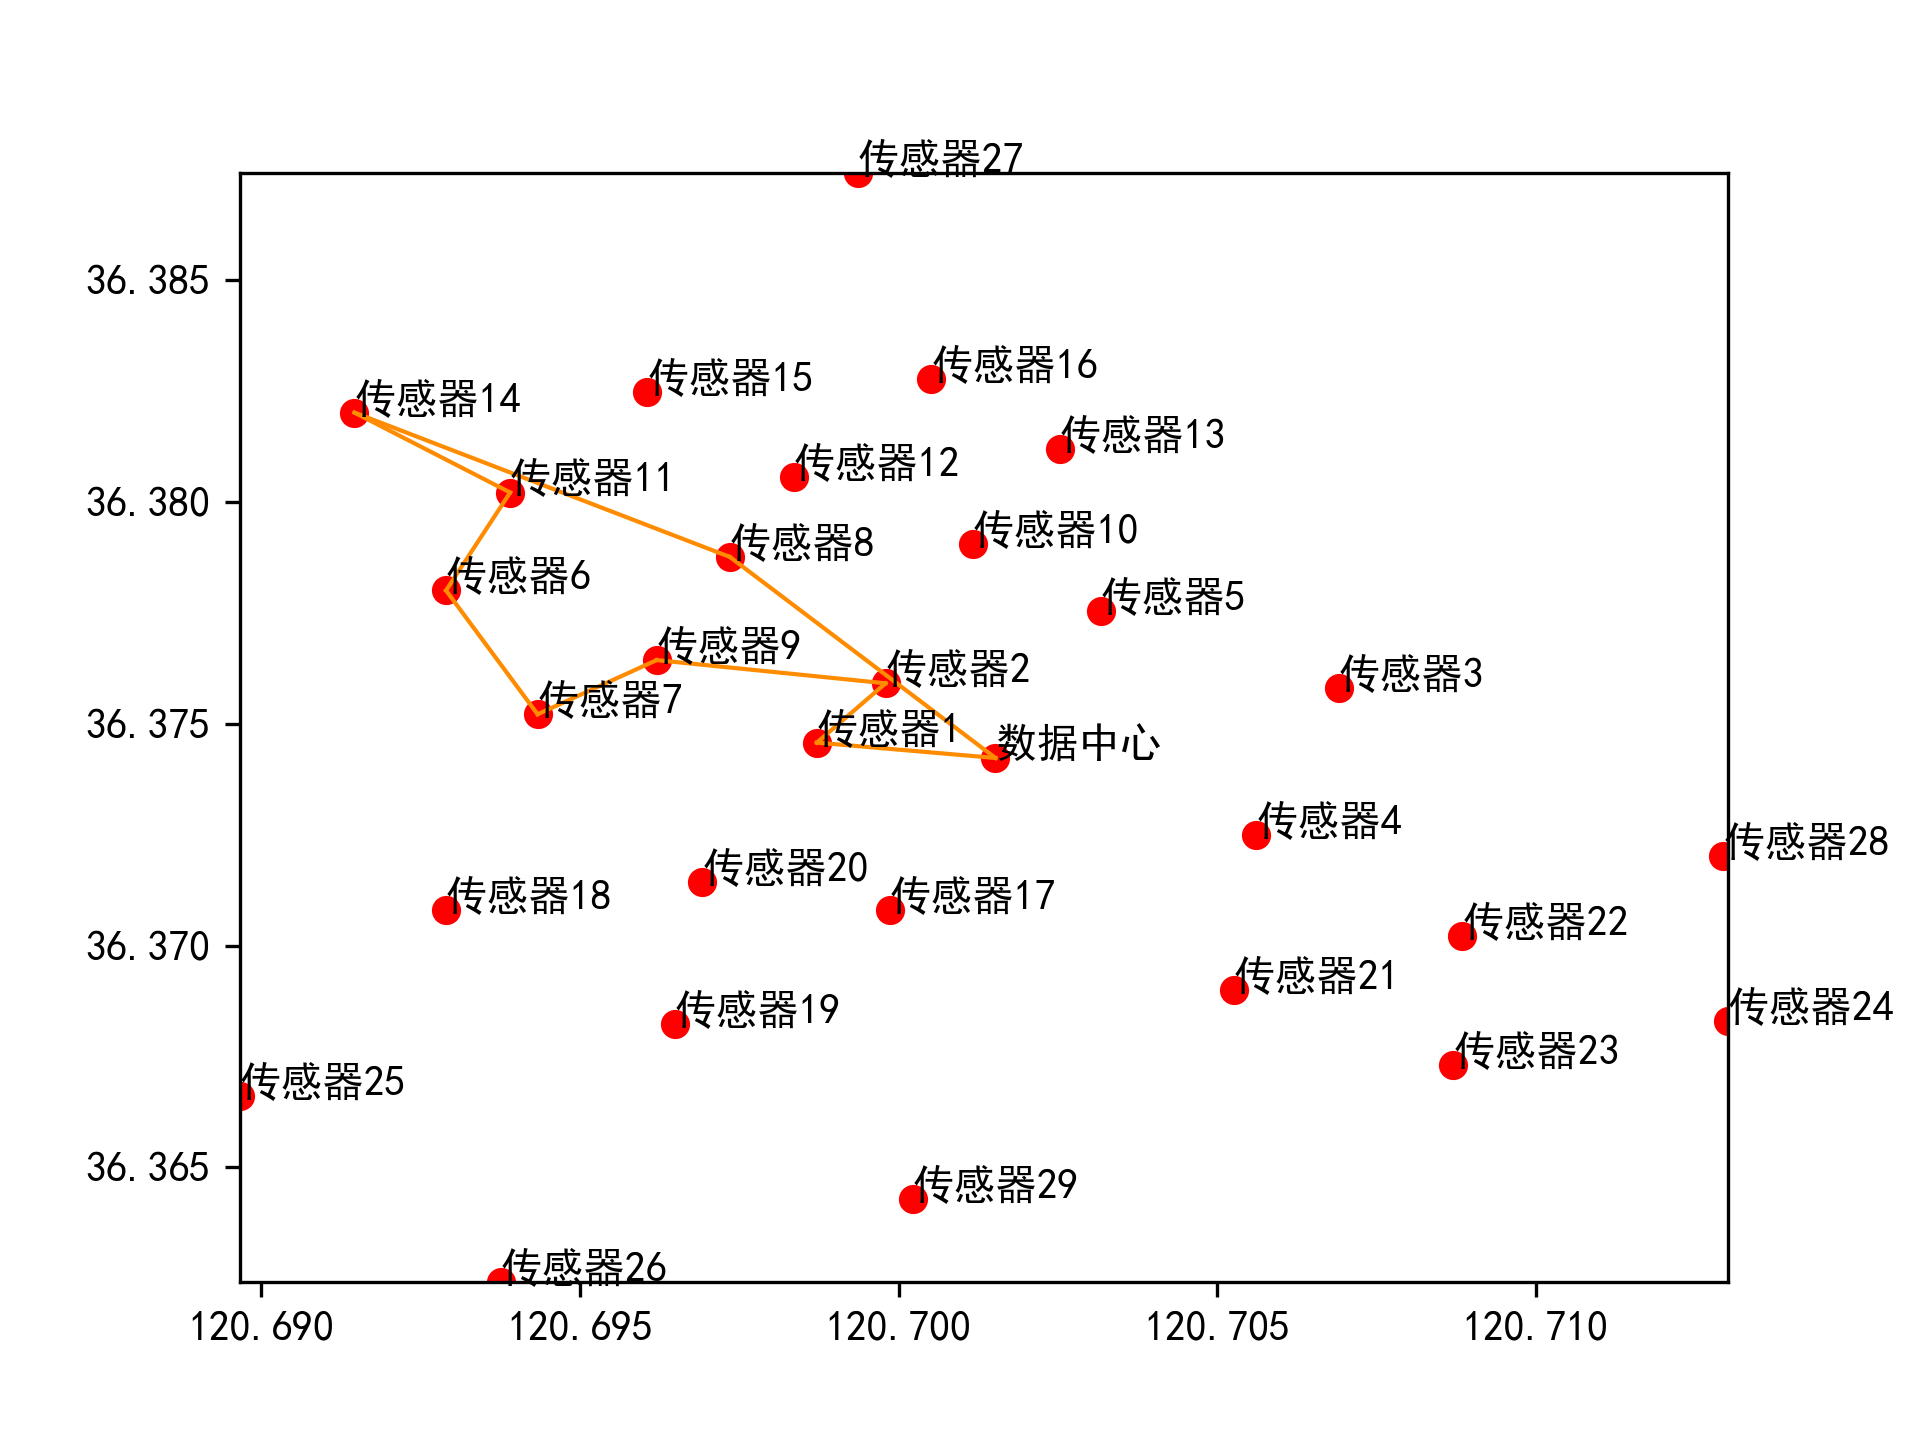
\includegraphics[width=3in]{figure/path_1.png}
        %\caption{fig1}
        \end{minipage}%
        }%
        \subfigure[移动充电器2]{
        \begin{minipage}[t]{0.5\linewidth}
        \centering
        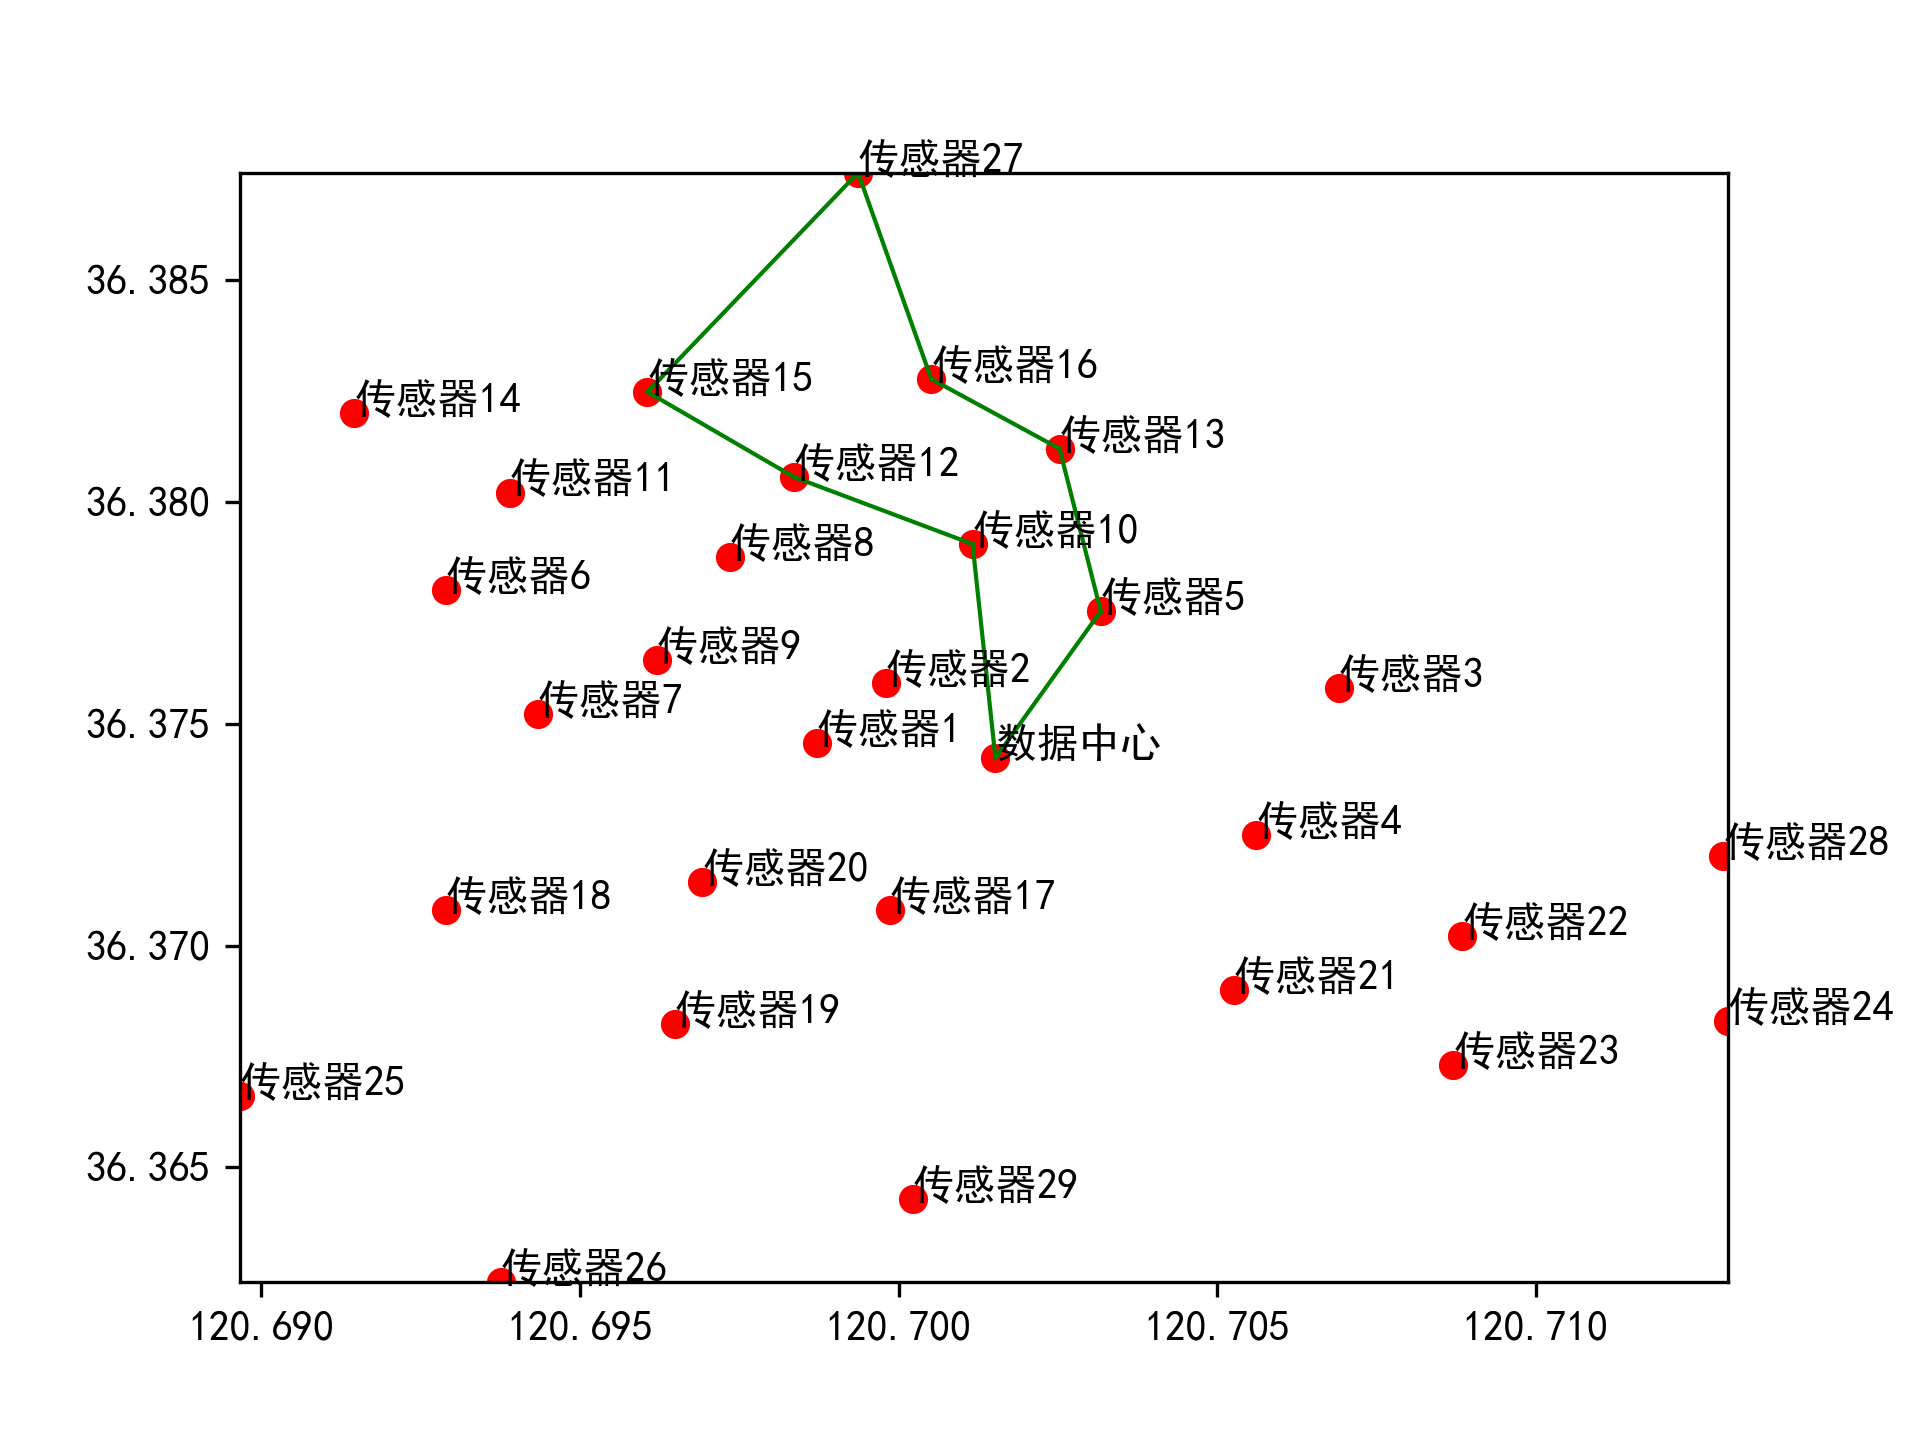
\includegraphics[width=3in]{figure/path_2.png}
        %\caption{fig2}
        \end{minipage}%
        }%
                         
        \subfigure[移动充电器3]{
        \begin{minipage}[t]{0.5\linewidth}
        \centering
        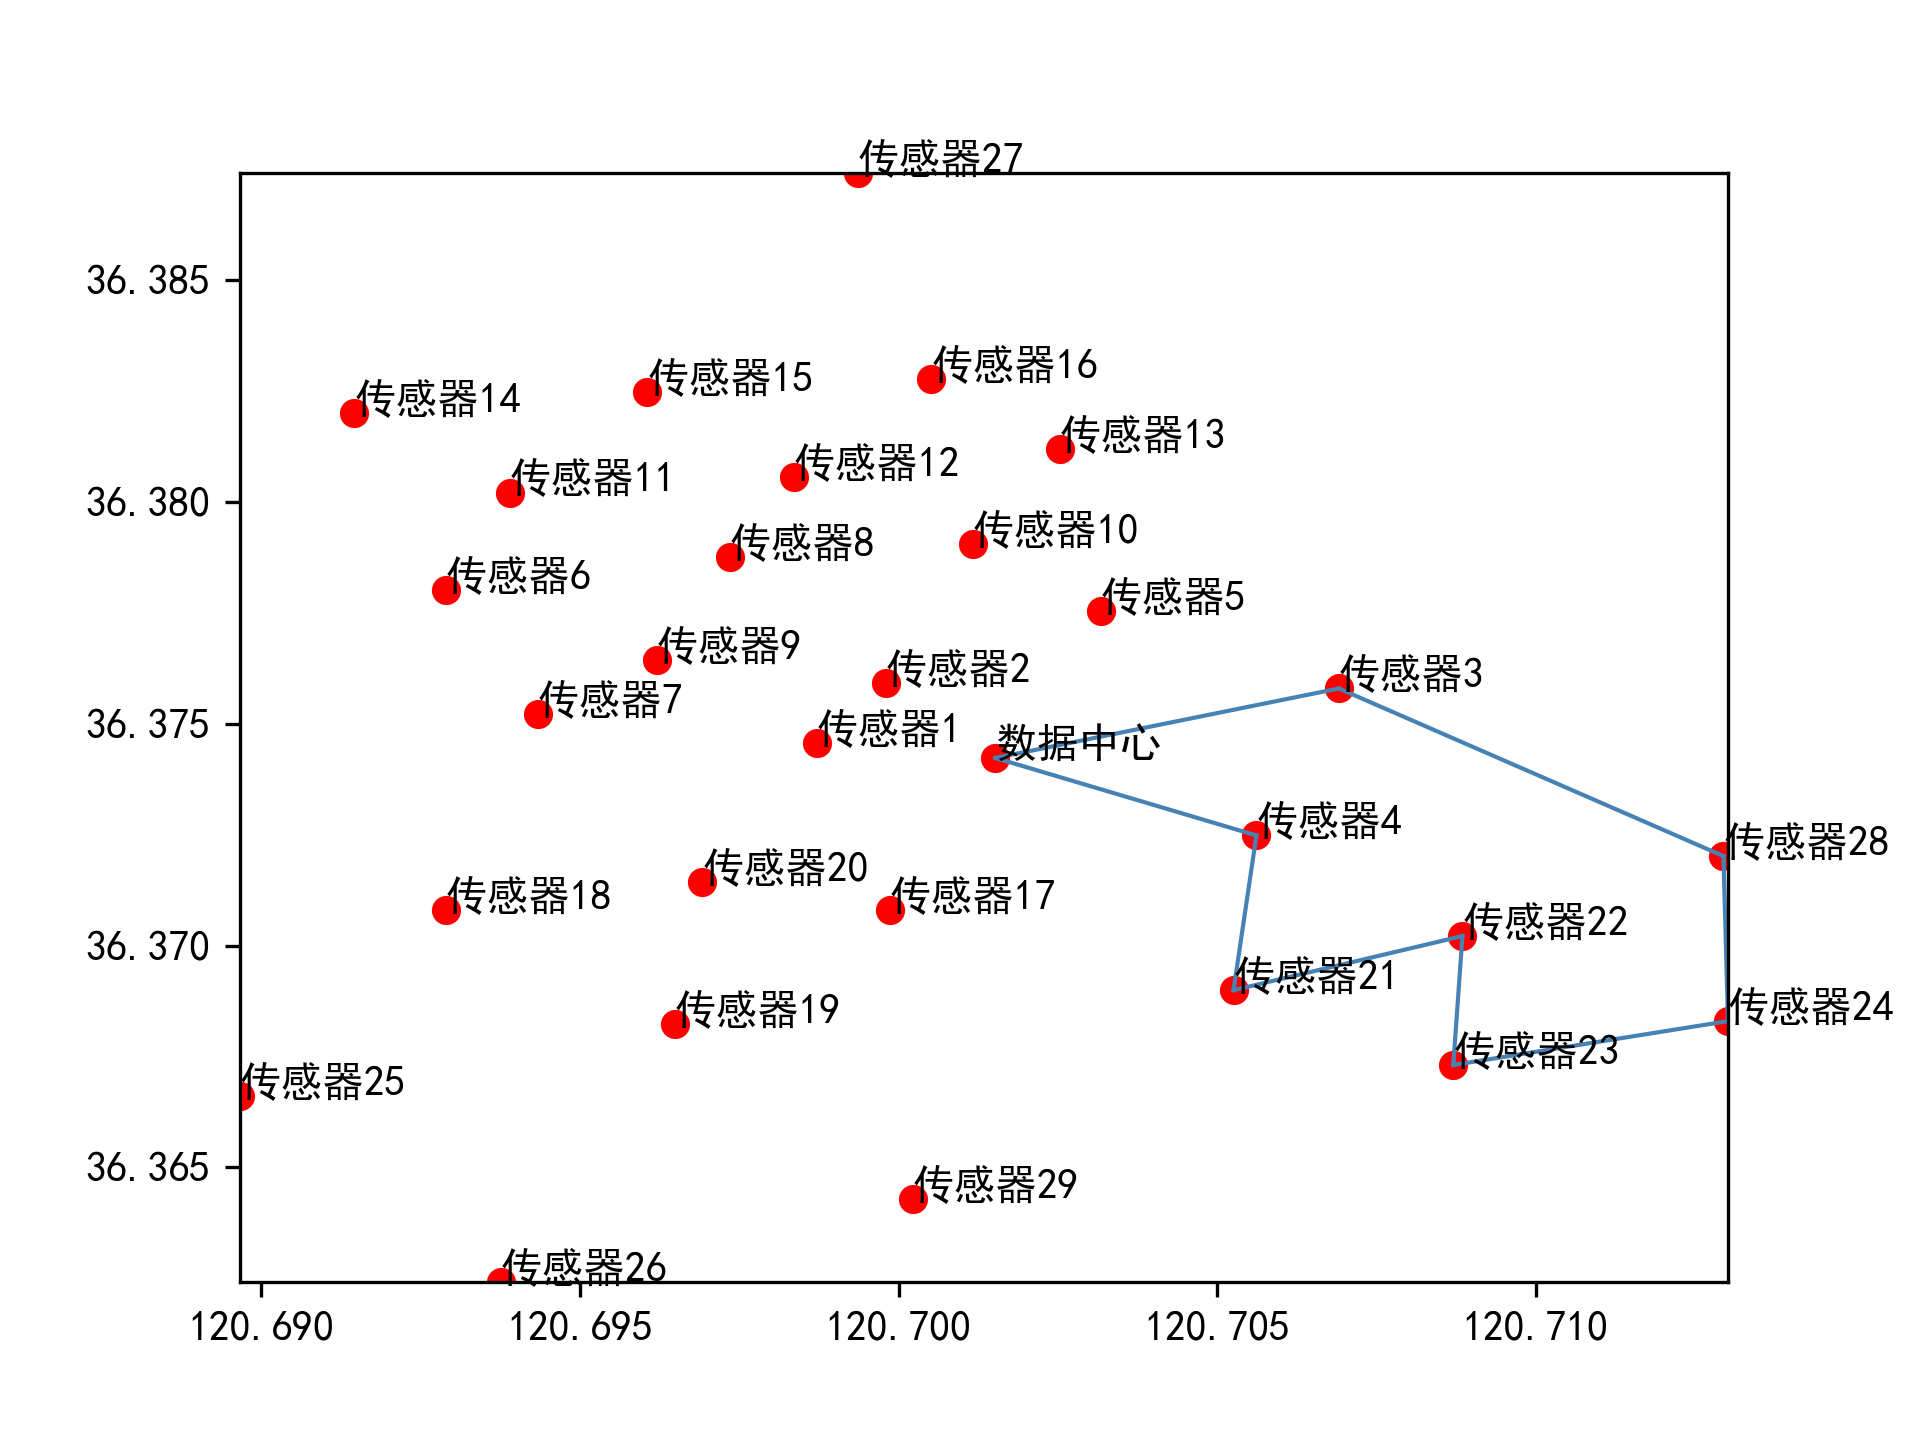
\includegraphics[width=3in]{figure/path_3.png}
        %\caption{fig2}
        \end{minipage}
        }%
        \subfigure[移动充电器4]{
        \begin{minipage}[t]{0.5\linewidth}
        \centering
        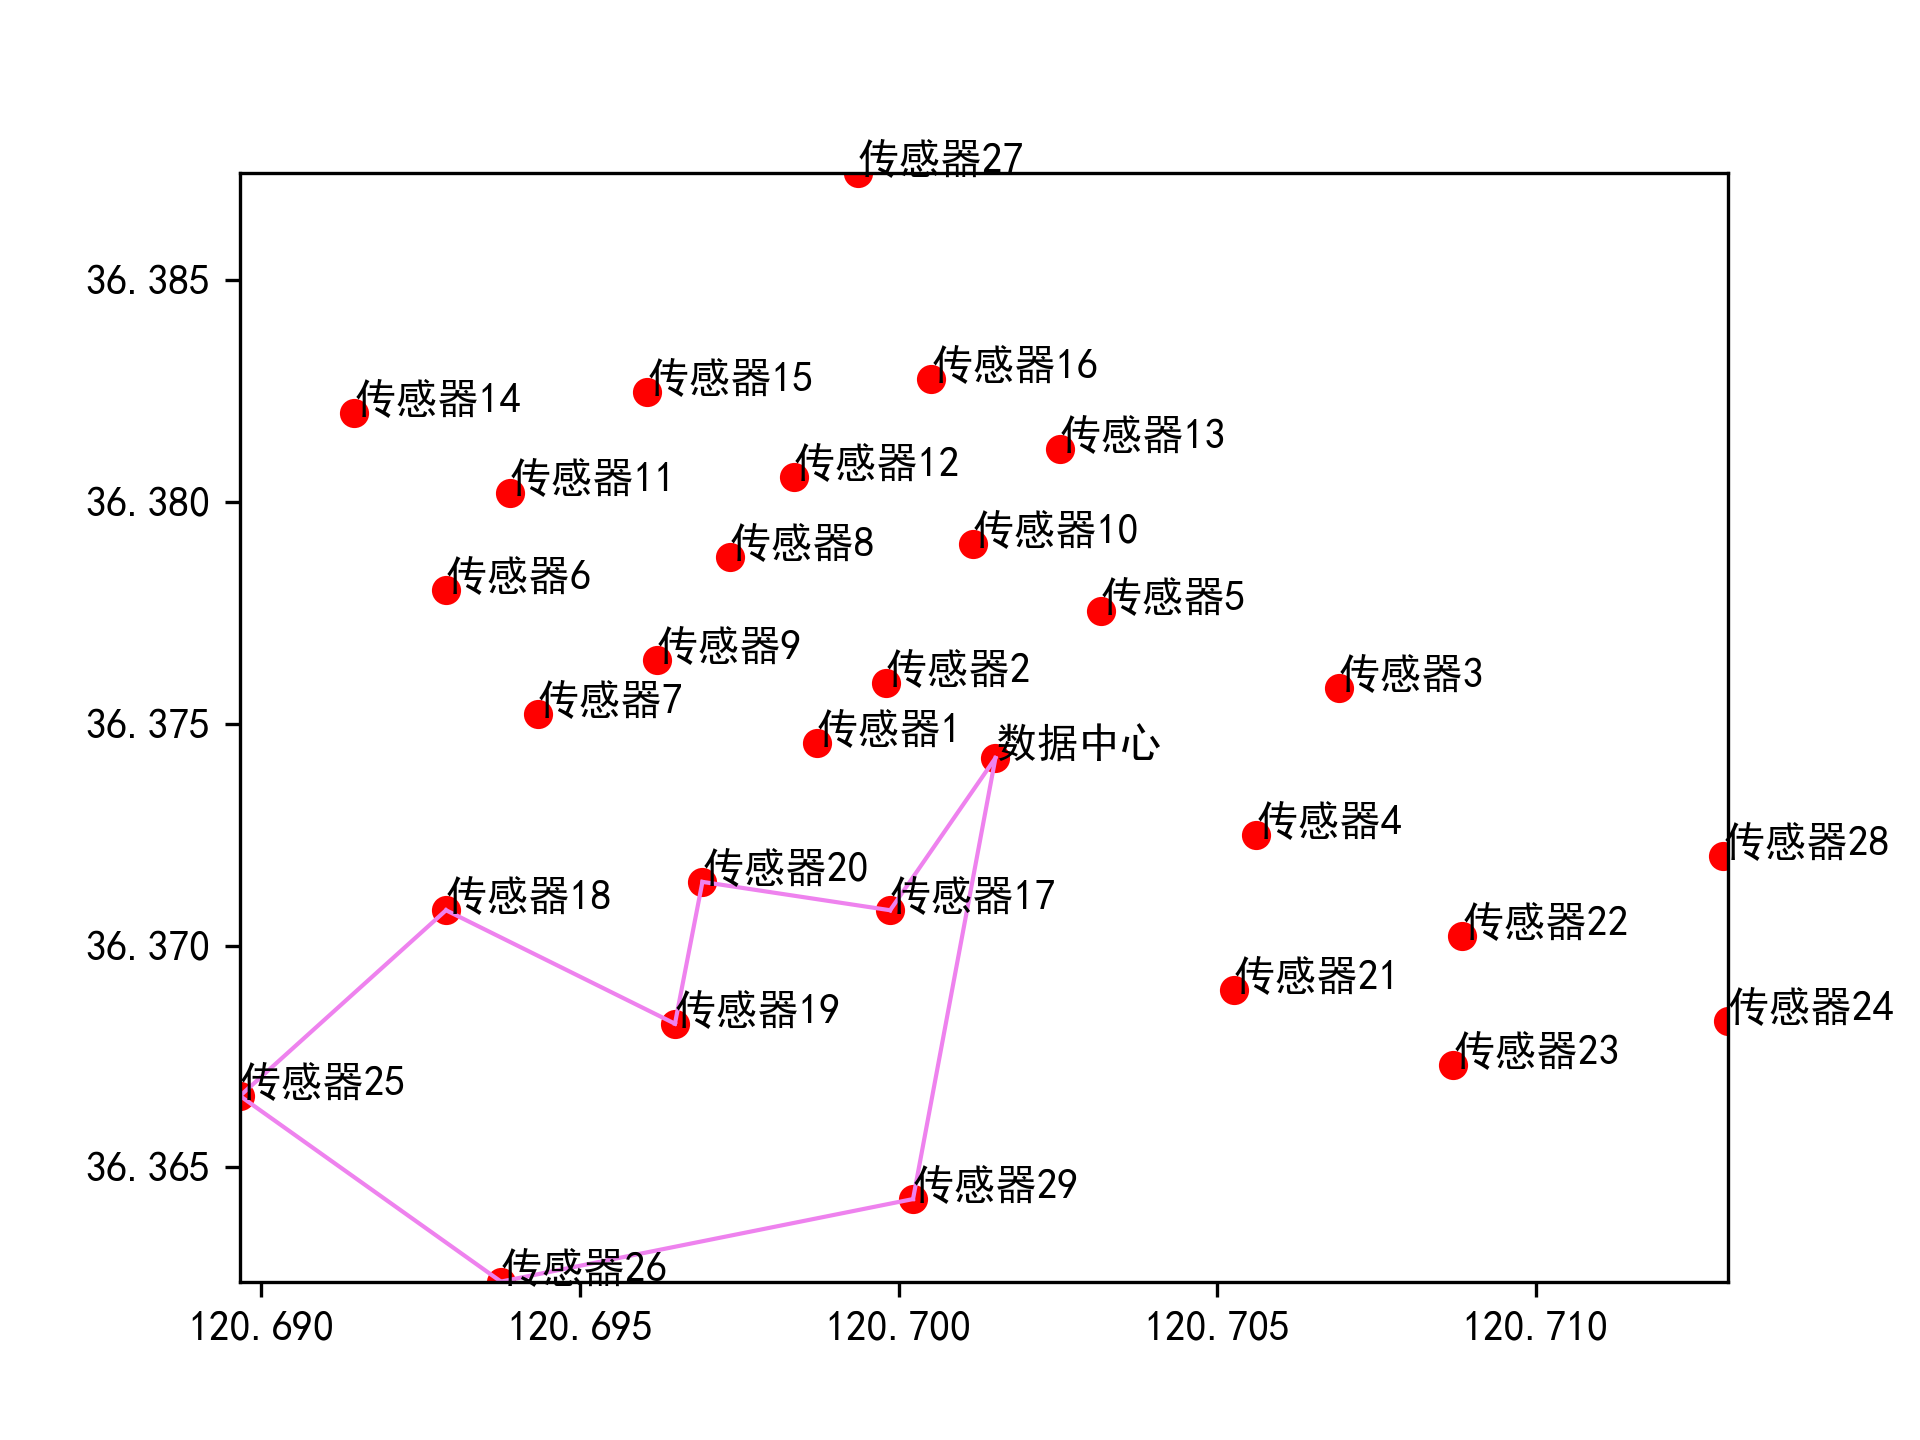
\includegraphics[width=3in]{figure/path_4.png}
        %\caption{fig2}
        \end{minipage}
        }%
        
        \centering
        \caption{移动充电器路径规划}
    \end{figure}
    由上图可知,四台移动充电器的路径用四种颜色表示,与问题一有较大的区别。显然,用四台移
    动充电器,可以大大减少所需的总路径。
    
    \subsection{电池最小容量的求解}
    这里我们参照问题二的解决方案,将四台移动充电器先分开求解,分别列出其约束条件并求解,
    最后整合成最终结果如下
    \begin{equation}
        C\geq f+\frac{1945.6}{v(\frac{1}{7.8}-\frac{7}{r})}
    \end{equation}

    \section{模型的推广与不足}
    在本题中,我们主要利用遗传算法对该问题进行了建模。主要的考虑是因为该问题的参数较多,
    如果利用常规方法,极有可能导致指数爆炸。因此,该启发式算法也为该模型的推广做了正向
    的贡献——可以适用于参数更多、更复杂的路线规划问题。

    然而,启发式算法也为该模型带来了很多不足:每一次运行的最终结果不能保证完全相同。也就
    是说,路线的规划并不能保证达到全局最优,而只能达到局部最优。这一点是至关重要的,有时
    一个次优的结果日积月累很有可能导致资源的极大浪费。

    因此,在后续我们需要对这一点不足作出进一步的改进。这里可以参考梯度下降法中的惯性参数,
    在模型达到局部最优时,可以利用其惯性来摆脱,继而进一步寻找全局最优解。

    \section*{附录}
    \subsection*{问题一:}
    \begin{python}
import numpy as np
import pandas as pd
from DW import *

class TSP(object):
    citys = np.array([])
    citys_name = np.array([])
    pop_size = 50
    c_rate = 0.7
    m_rate = 0.05
    pop = np.array([])
    fitness = np.array([])
    city_size = -1
    ga_num = 200
    best_dist = 1
    best_gen = []
    dw = Draw()

    def __init__(self, c_rate, m_rate, pop_size, ga_num):
        self.fitness = np.zeros(self.pop_size)
        self.c_rate = c_rate
        self.m_rate = m_rate
        self.pop_size = pop_size
        self.ga_num = ga_num

    def init(self):
        tsp = self
        # tsp.load_Citys()
        tsp.load_WSN()
        tsp.pop = tsp.creat_pop(tsp.pop_size)
        tsp.fitness = tsp.get_fitness(tsp.pop)
        tsp.dw.bound_x = [np.min(tsp.citys[:, 0]), np.max(tsp.citys[:, 0])]
        tsp.dw.bound_y = [np.min(tsp.citys[:, 1]), np.max(tsp.citys[:, 1])]
        tsp.dw.set_xybound(tsp.dw.bound_x, tsp.dw.bound_y)

    # --------------------------------------
    def creat_pop(self, size):
        pop = []
        for i in range(size):
            gene = np.arange(self.citys.shape[0])
            np.random.shuffle(gene)
            pop.append(gene)

        return np.array(pop)

    def get_fitness(self, pop):
        d = np.array([])
        for i in range(pop.shape[0]):
            gen = pop[i]  
            dis = self.gen_distance(gen)
            dis = self.best_dist / dis
            d = np.append(d, dis)
        return d

    def get_local_fitness(self, gen, i):
 
        di = 0
        fi = 0
        if i == 0:
            di = self.ct_distance(self.citys[gen[0]], self.citys[gen[-1]])
        else:
            di = self.ct_distance(self.citys[gen[i]], self.citys[gen[i - 1]])
        od = []
        for j in range(self.city_size):
            if i != j:
                od.append(self.ct_distance(self.citys[gen[i]], self.citys[gen[i - 1]]))
        mind = np.min(od)
        fi = di - mind
        return fi

    def EO(self, gen):
        local_fitness = []
        for g in range(self.city_size):
            f = self.get_local_fitness(gen, g)
            local_fitness.append(f)
        max_city_i = np.argmax(local_fitness)
        maxgen = np.copy(gen)
        if 1 < max_city_i < self.city_size - 1:
            for j in range(max_city_i):
                maxgen = np.copy(gen)
                jj = max_city_i
                while jj < self.city_size:
                    gen1 = self.exechange_gen(maxgen, j, jj)
                    d = self.gen_distance(maxgen)
                    d1 = self.gen_distance(gen1)
                    if d > d1:
                        maxgen = gen1[:]
                    jj += 1
        gen = maxgen
        return gen

    # -------------------------------------
    def select_pop(self, pop):
        best_f_index = np.argmax(self.fitness)
        av = np.median(self.fitness, axis=0)
        for i in range(self.pop_size):
            if i != best_f_index and self.fitness[i] < av:
                pi = self.cross(pop[best_f_index], pop[i])
                pi = self.mutate(pi)
                # d1 = self.distance(pi)
                # d2 = self.distance(pop[i])
                # if d1 < d2:
                pop[i, :] = pi[:]

        return pop

    def select_pop2(self, pop):
        probility = self.fitness / self.fitness.sum()
        idx = np.random.choice(np.arange(self.pop_size), size=self.pop_size, replace=True, p=probility)
        n_pop = pop[idx, :]
        return n_pop

    def cross(self, parent1, parent2):
        if np.random.rand() > self.c_rate:
            return parent1
        index1 = np.random.randint(0, self.city_size - 1)
        index2 = np.random.randint(index1, self.city_size - 1)
        tempGene = parent2[index1:index2]  # 交叉的基因片段
        newGene = []
        p1len = 0
        for g in parent1:
            if p1len == index1:
                newGene.extend(tempGene)  # 插入基因片段
            if g not in tempGene:
                newGene.append(g)
            p1len += 1
        newGene = np.array(newGene)

        if newGene.shape[0] != self.city_size:
            print('c error')
            return self.creat_pop(1)
            # return parent1
        return newGene

    def mutate(self, gene):
        """突变"""
        if np.random.rand() > self.m_rate:
            return gene
        index1 = np.random.randint(0, self.city_size - 1)
        index2 = np.random.randint(index1, self.city_size - 1)
        newGene = self.reverse_gen(gene, index1, index2)
        if newGene.shape[0] != self.city_size:
            print('m error')
            return self.creat_pop(1)
        return newGene

    def reverse_gen(self, gen, i, j):
        if i >= j:
            return gen
        if j > self.city_size - 1:
            return gen
        parent1 = np.copy(gen)
        tempGene = parent1[i:j]
        newGene = []
        p1len = 0
        for g in parent1:
            if p1len == i:
                newGene.extend(tempGene[::-1])  # 插入基因片段
            if g not in tempGene:
                newGene.append(g)
            p1len += 1
        return np.array(newGene)

    def exechange_gen(self, gen, i, j):
        c = gen[j]
        gen[j] = gen[i]
        gen[i] = c
        return gen

    def evolution(self):
        tsp = self
        for i in range(self.ga_num):
            best_f_index = np.argmax(tsp.fitness)
            worst_f_index = np.argmin(tsp.fitness)
            local_best_gen = tsp.pop[best_f_index]
            local_best_dist = tsp.gen_distance(local_best_gen)
            if i == 0:
                tsp.best_gen = local_best_gen
                tsp.best_dist = tsp.gen_distance(local_best_gen)

            if local_best_dist < tsp.best_dist:
                tsp.best_dist = local_best_dist
                tsp.best_gen = local_best_gen
                # tsp.dw.ax.cla()
                # tsp.re_draw()
                # tsp.dw.plt.pause(0.001)
            else:
                tsp.pop[worst_f_index] = self.best_gen
            print('gen:%d evo,best dist :%s' % (i, self.best_dist))

            tsp.pop = tsp.select_pop(tsp.pop)
            tsp.fitness = tsp.get_fitness(tsp.pop)
            for j in range(self.pop_size):
                r = np.random.randint(0, self.pop_size - 1)
                if j != r:
                    tsp.pop[j] = tsp.cross(tsp.pop[j], tsp.pop[r])
                    tsp.pop[j] = tsp.mutate(tsp.pop[j])
            #self.best_gen = self.EO(self.best_gen)
            tsp.best_dist = tsp.gen_distance(self.best_gen)

    def load_WSN(self, file='WSN_location.csv', delm=','):
        data = pd.read_csv(file, delimiter=delm, header=None).values
        self.citys = data[:, 1:]
        self.citys_name = data[:, 0]
        self.city_size = data.shape[0]

    def gen_distance(self, gen):
        distance = 0.0
        for i in range(-1, len(self.citys) - 1):
            index1, index2 = gen[i], gen[i + 1]
            city1, city2 = self.citys[index1], self.citys[index2]
            distance += np.sqrt((city1[0] - city2[0]) ** 2 + (city1[1] - city2[1]) ** 2)
        return distance

    def ct_distance(self, city1, city2):
        d = np.sqrt((city1[0] - city2[0]) ** 2 + (city1[1] - city2[1]) ** 2)
        return d

    def draw_citys_way(self, gen):
        '''
        根据一条基因gen绘制一条旅行路线
        :param gen:
        :return:
        '''
        tsp = self
        dw = self.dw
        m = gen.shape[0]
        tsp.dw.set_xybound(tsp.dw.bound_x, tsp.dw.bound_y)
        for i in range(m):
            if i < m - 1:
                best_i = tsp.best_gen[i]
                next_best_i = tsp.best_gen[i + 1]
                best_icity = tsp.citys[best_i]
                next_best_icity = tsp.citys[next_best_i]
                dw.draw_line(best_icity, next_best_icity)
        start = tsp.citys[tsp.best_gen[0]]
        end = tsp.citys[tsp.best_gen[-1]]
        dw.draw_line(end, start)

    def draw_citys_name(self, gen, size=5):
        '''
        根据一条基因gen绘制对应地点名称
        :param gen:
        :param size: text size
        :return:
        '''
        tsp = self
        m = gen.shape[0]
        tsp.dw.set_xybound(tsp.dw.bound_x, tsp.dw.bound_y)
        for i in range(m):
            c = gen[i]
            best_icity = tsp.citys[c]
            tsp.dw.draw_text(best_icity[0], best_icity[1], tsp.citys_name[c], 10)

    def re_draw(self):
        tsp = self
        tsp.dw.draw_points(tsp.citys[:, 0], tsp.citys[:, 1])
        tsp.draw_citys_name(tsp.pop[0], 8)
        tsp.draw_citys_way(self.best_gen)


def main():
    tsp = TSP(0.5, 0.1, 100, 500)
    tsp.init()
    tsp.evolution()
    tsp.re_draw()
    tsp.dw.plt.savefig('path.png', dpi=300)
    tsp.dw.plt.show()


if __name__ == '__main__':
    main()

    \end{python}

\subsection*{问题三:}
\begin{python}
import matplotlib.pyplot as plt
from matplotlib.lines import Line2D
import matplotlib.animation as animation

class Draw(object):
    bound_x = []
    bound_y = []

    def __init__(self):
        self.fig, self.ax = plt.subplots()
        self.plt = plt
        self.set_font()

    def draw_line(self, p_from, p_to):
        line1 = [(p_from[0], p_from[1]), (p_to[0], p_to[1])]
        (line1_xs, line1_ys) = zip(*line1)
        self.ax.add_line(Line2D(line1_xs, line1_ys, linewidth=1, color='green'))

    def draw_points(self, pointx, pointy):
        self.ax.plot(pointx, pointy, 'ro')

    def set_xybound(self, x_bd, y_bd):
        self.ax.axis([x_bd[0], x_bd[1], y_bd[0], y_bd[1]])

    def draw_text(self, x, y, text, size=8):
        self.ax.text(x, y, text, fontsize=size)

    def set_font(self, ft_style='SimHei'):
        plt.rcParams['font.sans-serif'] = [ft_style]
\end{python}
\end{document}